\documentclass[aspectratio=169]{beamer}
\usepackage[utf8]{inputenc}
\usepackage{tikz}
\usepackage{svg}
\usetheme[showmaxslides]{pureminimalistic}
\usepackage{appendixnumberbeamer}
\usepackage[backend=biber, doi=false, maxbibnames=2, maxcitenames=2,style=numeric, sorting=none, url=false, eprint=false]{biblatex}
\addbibresource{references.bib}

\renewcommand{\appendixname}{\texorpdfstring{\translate{appendix}}{appendix}}
\renewcommand{\logotitle}{\includesvg[width=.2\linewidth]{logos/unibo-logo.svg}}
\renewcommand{\logoheader}{}
\renewcommand{\logofooter}{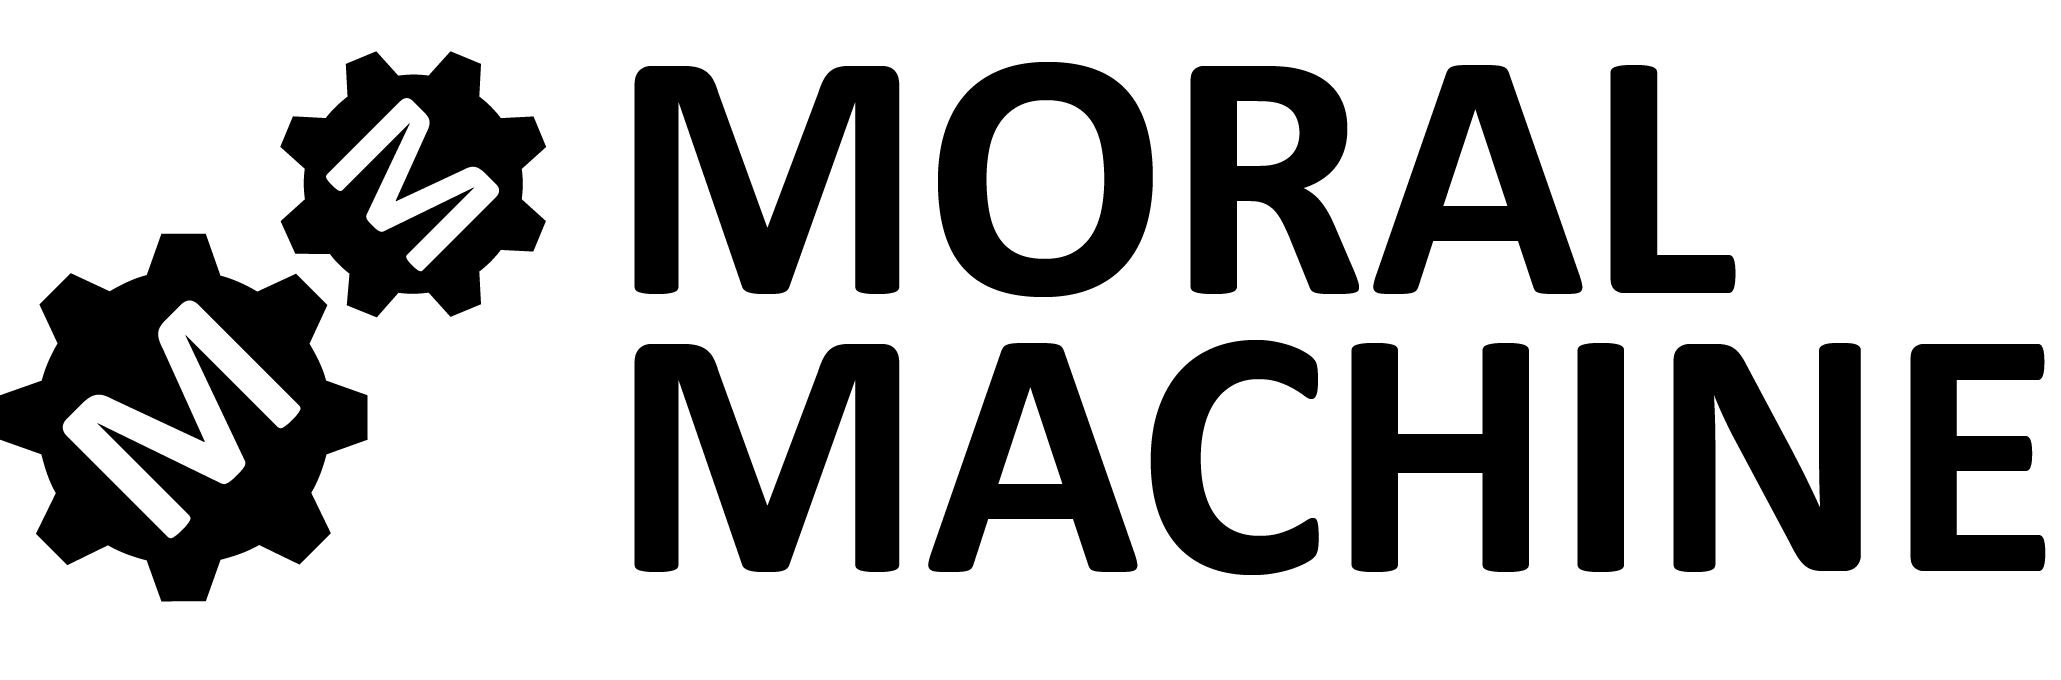
\includegraphics[width=.5\linewidth]{logos/mme-logo.png}}

\definecolor{bg}{RGB}{236, 240, 241}
\definecolor{text}{RGB}{52, 73, 94}
\definecolor{title}{RGB}{231, 76, 60}
\renewcommand{\beamerbgcolor}{bg}
\renewcommand{\beamertextcolor}{text}
\renewcommand{\beamertitlecolor}{title}

\title[MME]{The Moral Machine Experiment}
\author{Leonardo Calbi, Lorenzo Cellini, Alessio Falai\\}
\institute{Alma Mater Studiorum - University of Bologna}
\date{\today}

% Section slides with title only
\AtBeginSection[]{
  \begin{frame}[plain, noframenumbering]
    \centering
    \vfill
    {\usebeamerfont{title} \insertsectionhead\par}
    \vfill
  \end{frame}
}

\begin{document}
\maketitle

% TOC
\begin{frame}[plain, noframenumbering]{Outline}
    \tableofcontents
\end{frame}

% Introduction
\section{Why ethics matters for autonomous cars}
\begin{frame}
    Introduction
\end{frame}

\section{The Moral Machine Experiment}

\begin{frame}
    \frametitle{Introduction}
    \begin{columns}
        \begin{column}{0.6\linewidth}
            \begin{itemize}
                \item MME \cite{mme} is an online experimental platform, designed to gauge social expectections about how autonomous vehicles should solve moral dilemmas
                \item It gathered almost $40M$ decisions from $233$ different countries in $10$ languages
                \item What would you want an AV to do if its brakes failed?
                \begin{itemize}
                    \item Keep the lane and hit pedestrians on the road?
                    \item Swerve and hit pedestrians on the other lane?
                    \item Hit a barrier with the car?
                \end{itemize}
                \item What would happen to the chosen characters?
                \begin{itemize}
                    \item Skull $\rightarrow$ death
                    \item Medical cross $\rightarrow$ injury
                    \item Question mark $\rightarrow$ unknown
                \end{itemize}
            \end{itemize}
        \end{column}
        \begin{column}{0.4\linewidth}
            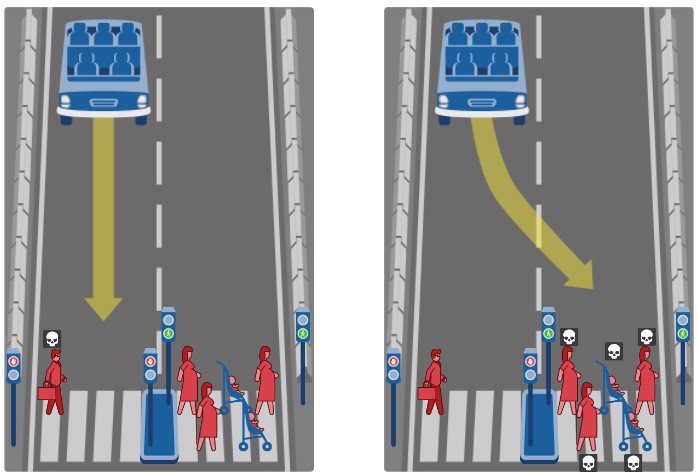
\includegraphics[width=1.0\linewidth]{assets/example-mme.jpg}
        \end{column}
    \end{columns}
\end{frame}

\begin{frame}
    \frametitle{Analysis framework}
    \begin{enumerate}
        \item Sparing humans (versus pets)
        \item Staying on course (versus swerving)
        \item Sparing passengers (versus pedestrians)
        \item Sparing more lives (versus fewer lives)
        \item Sparing men (versus women)
        \item Sparing the young (versus the elderly)
        \item Sparing pedestrians who cross legally (versus jaywalking)
        \item Sparing the fit (versus the less fit)
        \item Sparing those with higher social status (versus lower social status)
    \end{enumerate}
\end{frame}

\begin{frame}
    \frametitle{Relative importance}
    \begin{figure}
        \center
        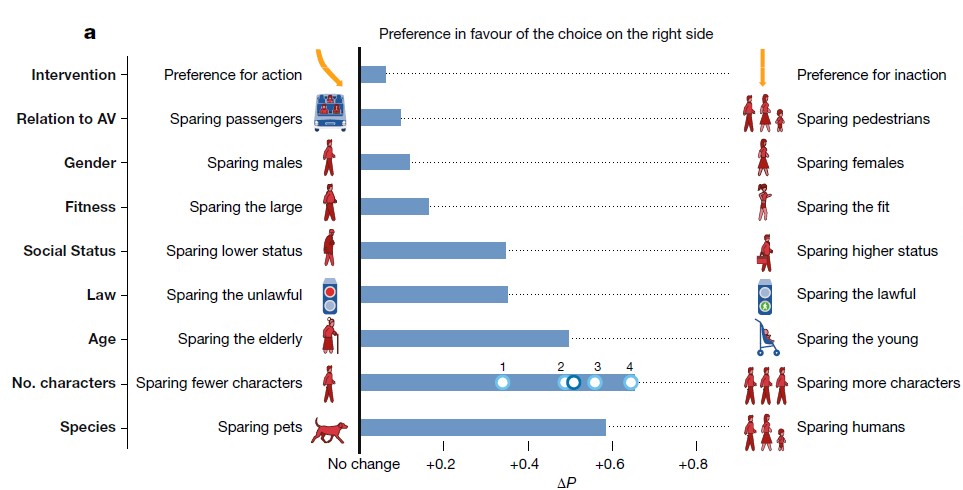
\includegraphics[width=0.8\linewidth]{assets/relative-importance-mme.jpg}
        \caption{In each row, $\Delta p$ is the difference between the probability of sparing characters possessing the attribute on the right, and the probability of sparing characters possessing the attribute on the left, aggregated over all other attributes}
    \end{figure}
\end{frame}

\begin{frame}
    \frametitle{Individual variations}
    \begin{columns}
        \begin{column}{0.6\linewidth}
            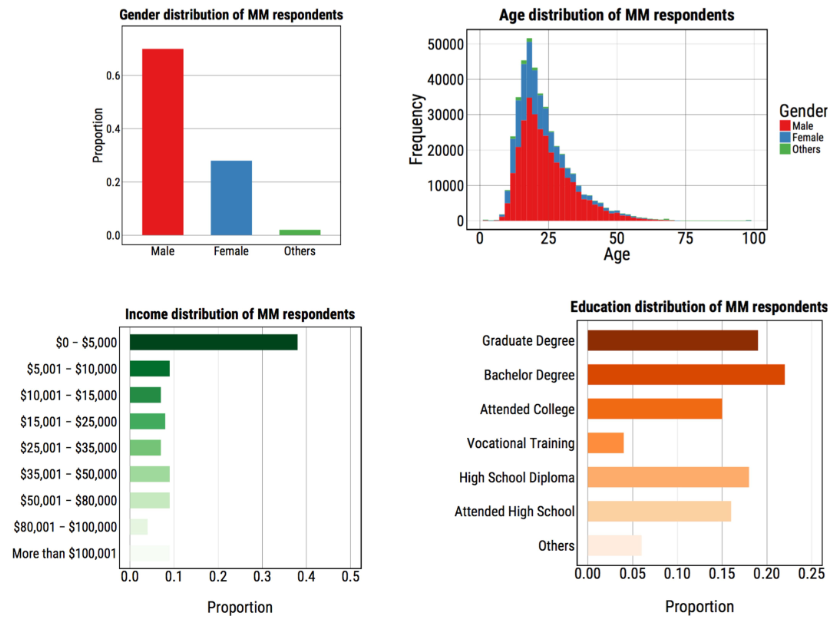
\includegraphics[width=1.0\linewidth]{assets/demographics-mme.png}
        \end{column}
        \begin{column}{0.4\linewidth}
            \begin{itemize}
                \item Subgroup of Moral Machine users ($492921$) who completed the optional demographic survey on age, education, gender, income, and political and religious views
                \item Including all six characteristic variables in regression-based estimators of each of the nine attributes shows that individual variations have no sizable impact on any of them (all below 0.1 $\rho$-value)
            \end{itemize}
        \end{column}
    \end{columns}
\end{frame}

\begin{frame}
    \frametitle{Hierarchical clustering of countries}
    \begin{columns}
        \begin{column}{0.6\linewidth}
            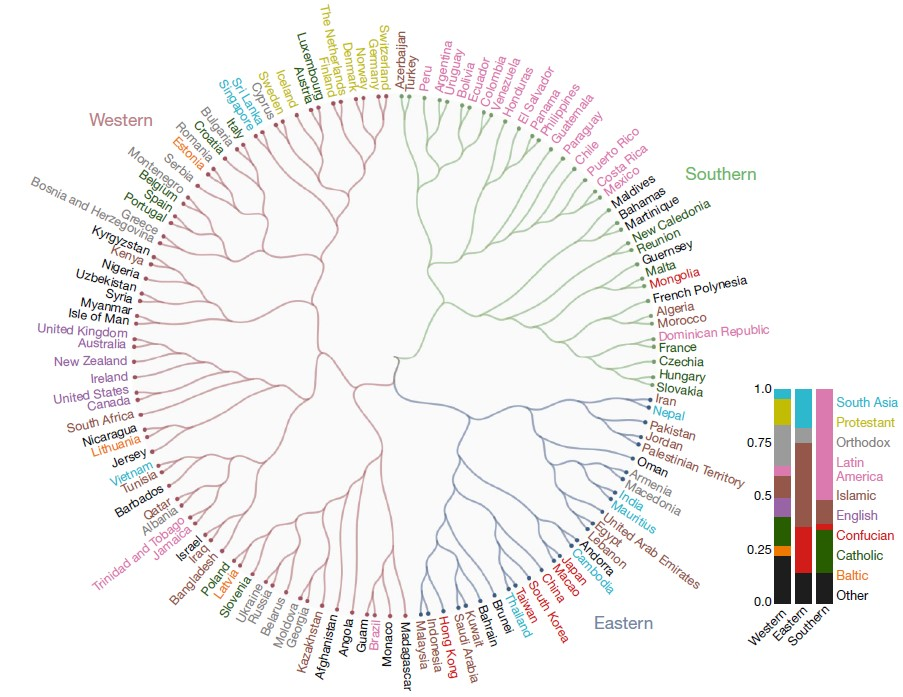
\includegraphics[width=1.0\linewidth]{assets/countries-mme.jpg}
        \end{column}
        \begin{column}{0.4\linewidth}
            \begin{itemize}
                \item \textbf{Western cluster}: NA and EU countries (Protestant, Catholic, and Orthodox Christian cultural groups)
                \item \textbf{Eastern cluster}: countries such as Japan, Taiwan, Indonesia, Pakistan and Saudi Arabia (Confucianist and Islamic cultural groups)
                \item \textbf{Southern cluster}: consists of the Latin American countries of Central and South America, in addition to some countries that are characterized in part by French influence
            \end{itemize}
        \end{column}
    \end{columns}
\end{frame}

\begin{frame}
    \frametitle{Cluster preferences}
    \begin{figure}
        \center
        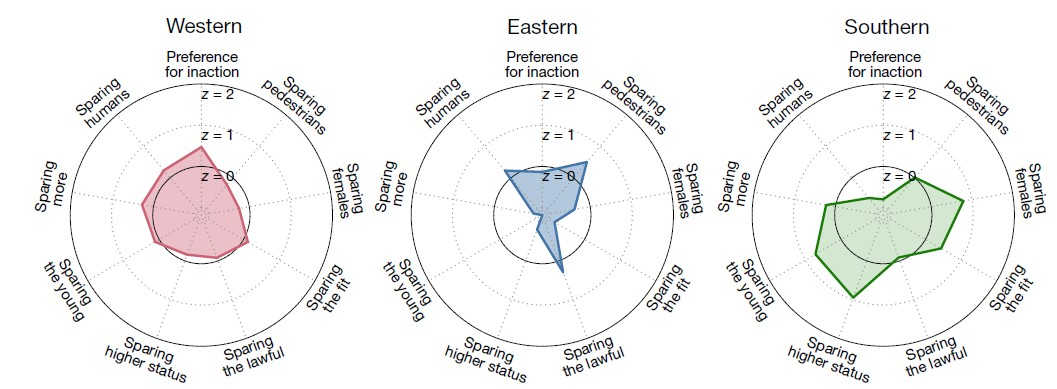
\includegraphics[width=0.8\linewidth]{assets/clusters-mme.jpg}
    \end{figure}
    \bigskip
    \begin{itemize}
        \item Systematic differences between individualistic and collectivistic cultures (young vs old and less vs more)
        \item Certain characters are preferred for demographic reasons (male vs female and rich vs poor)
        \item Choices related to one's perception of law and quality of rules and institutions (pedestrian vs jaywalker)
    \end{itemize}
\end{frame}

\begin{frame}
    \frametitle{Discussion}
    \begin{enumerate}
        \item Three strong preferences: sparing human lives, more lives and young lives
        \item Some preferences based on gender or social status vary considerably across countries, and appear to reflect underlying societal level preferences for egalitarianism
        \item Samples are not guaranteed to be representative: this means that policymakers should not embrace MME results as the final word on societal preferences
        \item Technologically unrealistic assumptions, such as the absence of uncertainty over character classification (adult vs children) and life/death outcomes 
    \end{enumerate}
\end{frame}

\section{Arguments against MME}
\begin{frame}
    \frametitle{Weak points of MME}
    \begin{itemize}
        \item The apparent preference for inequality in MME results is driven by the specific "trolley-type" paradigm used by the experimenters
        \item MME concludes that people want AVs to make decisions about who to kill on the basis of personal features, including physical fitness, age, status and gender
        \begin{itemize}
            \item This conclusion contradicts well-documented ethical preferences for equal treatment across demographic features and identities
            \item Ignoring personal traits is also more consistent with the current technical capacities of AVs
        \end{itemize}
    \end{itemize}
\end{frame}

\begin{frame}
    \frametitle{Experiments}
    To prove the ineffectiveness of MME, \citeauthor{against-mme} realized three different experiments
    \begin{enumerate}
        \item People were randomly assigned either a forced inequality question (replication of MME in a simplified setting) or an equality-allowed condition (\textit{"treat the lives of group A and B equally"})
        \item Similar to the first study, with a modified third option: \textit{"AVs should decide who to save and who to kill without considering their personal features"}
        \item Participants chose which of the two AVs should be allowed on the road: AVs based solely on structural features or both structural and personal features revealed by MME
    \end{enumerate}
\end{frame}

\begin{frame}
    \frametitle{First experiment}
    \begin{columns}
        \begin{column}{0.6\linewidth}
            \begin{itemize}
                \item Quasi-representative sample: $1174$ US participants and $1178$ UK participants using an online survey system
                \item Results from the forced inequality condition closely match the global effects of the MME
                \item People overwhelmingly selected the third option when it was available, revealing that they want autonomous vehicles to treat people equally
                \begin{itemize}
                    \item For example, when forced to choose between men and women, $87.7\%$ chose to save women, but $97.9\%$ of people actually preferred to treat both groups equally
                \end{itemize}
            \end{itemize}
        \end{column}
        \begin{column}{0.4\linewidth}
            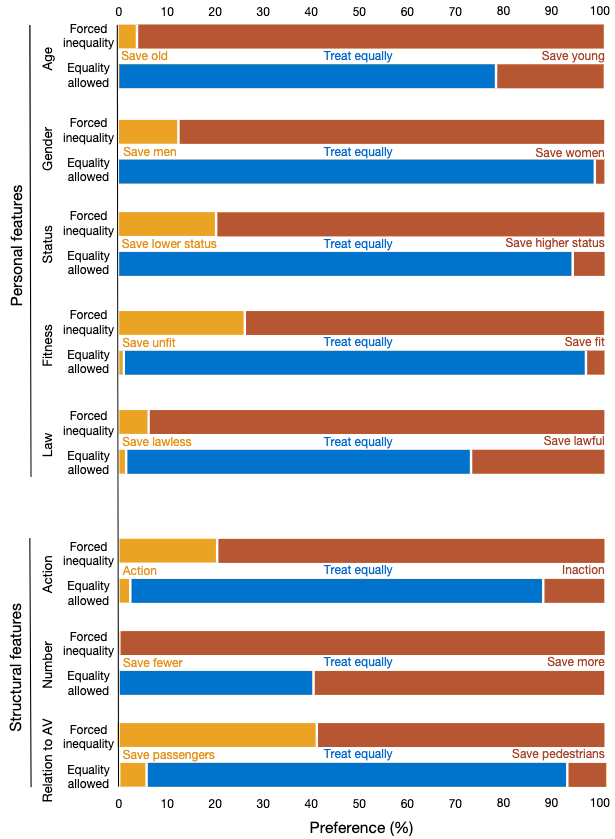
\includegraphics[width=0.9\linewidth]{assets/against-mme-first-experiment.png}
        \end{column}
    \end{columns}
\end{frame}


\begin{frame}
    \frametitle{Second experiment}
    \begin{itemize}
        \item Sample: $843$ US participants from an online panel
        \item Study 2 rules out the concern of whether participants preferred the "treat equally" option in study 1 simply because it failed to mention killing
        \item Consistent with study 1, people expressed a robust preference for AVs to treat people equally by ignoring personal features
        \begin{itemize}
            \item For example, people preferred self-driving cars to not consider gender ($92.6\%$), fitness ($88.8\%$) or status ($84.7\%$)
            \item The only substantial departure from study 1 was lawfulness: $53.1\%$ of people preferred to spare law abiders over law breakers
        \end{itemize}
    \end{itemize}
\end{frame}

\begin{frame}
    \frametitle{Third experiment}
    \begin{itemize}
        \item Sample: $993$ US participants from an online panel
        \item Personal features (law, fitness, status, gender and age) and structural features (passengers/pedestrians, fewer/more and action/inaction)
        \item Results show that $89.9\%$ of participants chose the structural-features-only car, once again expressing a desire for AVs that ignore personal features in ethical dilemmas
    \end{itemize}
\end{frame}

\begin{frame}
    \frametitle{Reply from MME's authors}
    \begin{itemize}
        \item \citeauthor{against-mme} asked eight separate questions about general policy preferences (one per dimension), while MME had users go through multiple pairs of nine-dimensional outcomes
        \item The MME approach allows us to measure the weight of different moral priorities when pitted against each other, rather than considered in isolation, but participants cannot explicitly state that one dimension (for example, age) should not be taken into account
        \item The approach used by \citeauthor{against-mme} is more sensitive to social desirability, experimental demands and framing effects w.r.t. MME
        \item MME's authors (\citeauthor{mme}) tried an approach similar to the one by \citeauthor{against-mme} that went unpublished
    \end{itemize}
\end{frame}

\begin{frame}
    \frametitle{MME unpublished experiment}
    \begin{columns}
        \begin{column}{0.6\linewidth}
            \begin{itemize}
                \item $585531$ MME users were taken to a page where they could position one slider for each of the nine dimensions explored by the Moral Machine: users could move the slider to express how important this dimension should be
                \item Values on the sliders were initialized based on user's decisions on MME questions
                \item Participants could easily express an equality preference by positioning the slider at the midpoint of the scale 
                \begin{itemize}
                    \item This is a continuos alternative to the method used by \citeauthor{against-mme}, which relies on visual (instead of textual) cues
                \end{itemize}
                \item A clear deviation towards equality from standard MME results is mainly observed on social status preference and over other dimesions with a lower intensity
            \end{itemize}
        \end{column}
        \begin{column}{0.4\linewidth}
            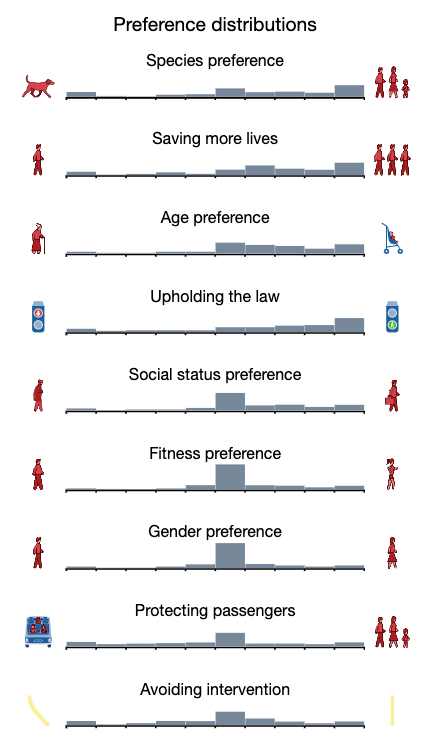
\includegraphics[width=0.7\linewidth]{assets/reply-against-mme-experiment.png}
        \end{column}
    \end{columns}
\end{frame}

\section{Conclusions}
\begin{frame}
    \cite{mme}
\end{frame}

\appendix
\begin{frame}[plain, noframenumbering]{References}
    \printbibliography
\end{frame}

\section*{Backup frames}
\begin{frame}[plain, noframenumbering]
    \centering
    \vfill
    {\usebeamerfont{title} Backup frames}
    \vfill
\end{frame}

\begin{frame}{Backup demo}
    Demo
\end{frame}

\end{document}
